\section{Desired model}

The desired model shall provide a setting for which we can explore fundamental resource and performance properties of the \xcloud{} system paradigm with mobile \ues{}. The mobile \ues{}, radio access network, and service application will subject the \dcs{} with a load characteristic for generic mobile phone traffic and the type of services that plausible might be deployed to the \xcloud{}.

\begin{figure}[tb]
	\centering
	\includegraphics[width=\linewidth]{fig_system_model.eps} 
	\caption{System model}
	\label{fig:system_model}
\end{figure}

As the topology of any future \xcloud{} or proposed forthcoming mobile networks is yet to be determined, in this paper we propose a generic telecom infrastructure model that disregards generational specific properties such as those found in the physical layer and radio resource load-balancing methods. These properties are not system variables at the abstraction level the \xcloud needs to be modelled in this paper. Nevertheless, conceivably, and in order to confine the geographic domain of the model, the model adheres to current general LTE cell planing practices \cite{salo2010practical}, see Figure \ref{fig:system_model}.

In order to be able to explore the fundamental effects of mobility on the performance of an \xcloud service in the generic case, the model does not adhere to any soci-demographic patterns or urban topologies. With out any geographic bias, the mobile network base stations are uniformly distributed across its 2-dimensional domain.

Similarly, in order to represent the variety of possible services, the service model shall generate traffic that is characteristic for an active, generic, \ue{}. Additionally, the generated traffic shall be provided by a stochastic process that is also independent of location.

Themobility model, the service model, and the uniformly distributed mobile network provides the modelled \dcs{} withc a characteristic workload. It is worth reiterating that the traffic load is more relevant to our investigation than specific topological and network properties.

The \dc{} model will host multiple VMs that will process the arriving requests corresponding to its service commitment. Additionally, when a VM is migrated between \dcs{} it shall incur a load on both \dcs{}. Furthermore, the resources within a \dc{} are shared amongst the hosted VMs. The amount of compute resources dedicated to one service is thus proportional to the number of services hosted in that \dc{}.  Minute memory management, interference, and cross-talk effects are not fundamental performance properties at this scale and are therefore not modelled.
